\documentclass[12pt,a4paper]{article}
\usepackage[utf8]{inputenc}
\usepackage{geometry}
\usepackage{titlesec} % For customizing section titles
\usepackage{graphicx} % For images
\usepackage{hyperref} % For hyperlinks
\usepackage{fancyhdr} % For fancy headers and footers
\usepackage{lipsum} % For generating dummy text
\usepackage{graphicx}
\usepackage{subcaption}
\usepackage{dirtree}

% Set page geometry
\geometry{left=2.5cm, right=2.5cm, top=2.5cm, bottom=2.5cm}

% Set up hyperref
\hypersetup{
    colorlinks=true,
    allcolors=blue,
    linkcolor=black,
    filecolor=cyan,
    urlcolor=blue,
}

% Customize section titles
\titleformat{\section}{\large\bfseries}{\thesection}{1em}{}
\titleformat{\subsection}{\normalsize\bfseries}{\thesubsection}{1em}{}

% Setup headers and footers
\pagestyle{fancy}
\fancyhf{}
\rhead{3D printing defect detection}
\lhead{Data provisioning}
\rfoot{Page \thepage}

% Title and author
\title{{\textbf{Data provisioning for 3D printing defect (spaghetti) detection}\\ {\small Simplified version}}}

\author{Michal Raczkowski}
\date{15-01-2024}

\begin{document}

\maketitle
\thispagestyle{empty} % Remove header/footer for the first page

% Insert table of contents
\newpage
\tableofcontents
\newpage

\setcounter{page}{1} % Start page numbering from here

\section{Introduction}
This document outlines the process of data collection, processing, and labeling for training a YOLO algorithm in detecting defects in 3D printing, with a focus on the "spaghetti" issue.

\section{Data Requirements}
The YOLO algorithm requires labeled images that display the "spaghetti" defect in 3D prints. These images must be open-source and correctly formatted.

\section{Data Collection}
Data is sourced from homemade images and open-source online datasets, ensuring a focus on the "spaghetti" defect.

\section{Data Understanding}
The dataset comprises photos showing various 3D printing defects. The selection process involves choosing images that specifically display the "spaghetti" defect.
\begin{figure}[h]
    \centering
    \begin{subfigure}[b]{0.45\textwidth}
        \centering
        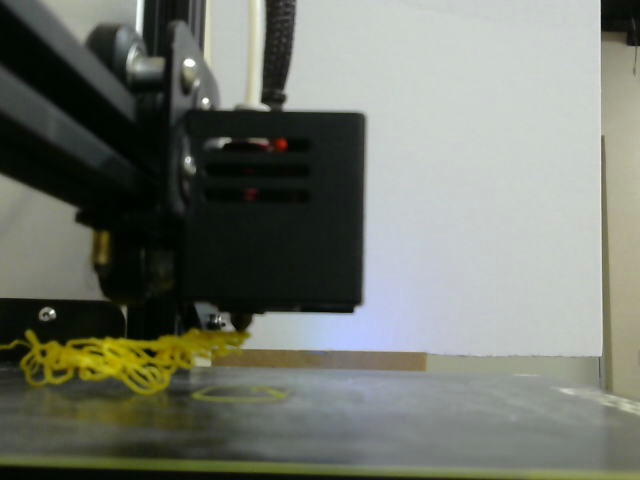
\includegraphics[width=\textwidth]{no_support_0.jpg}
        \caption{"Spaghetti" issue\cite{onlineOpenSource1}}
        \label{fig:image1}
    \end{subfigure}
    \begin{subfigure}[b]{0.45\textwidth}
        \centering
        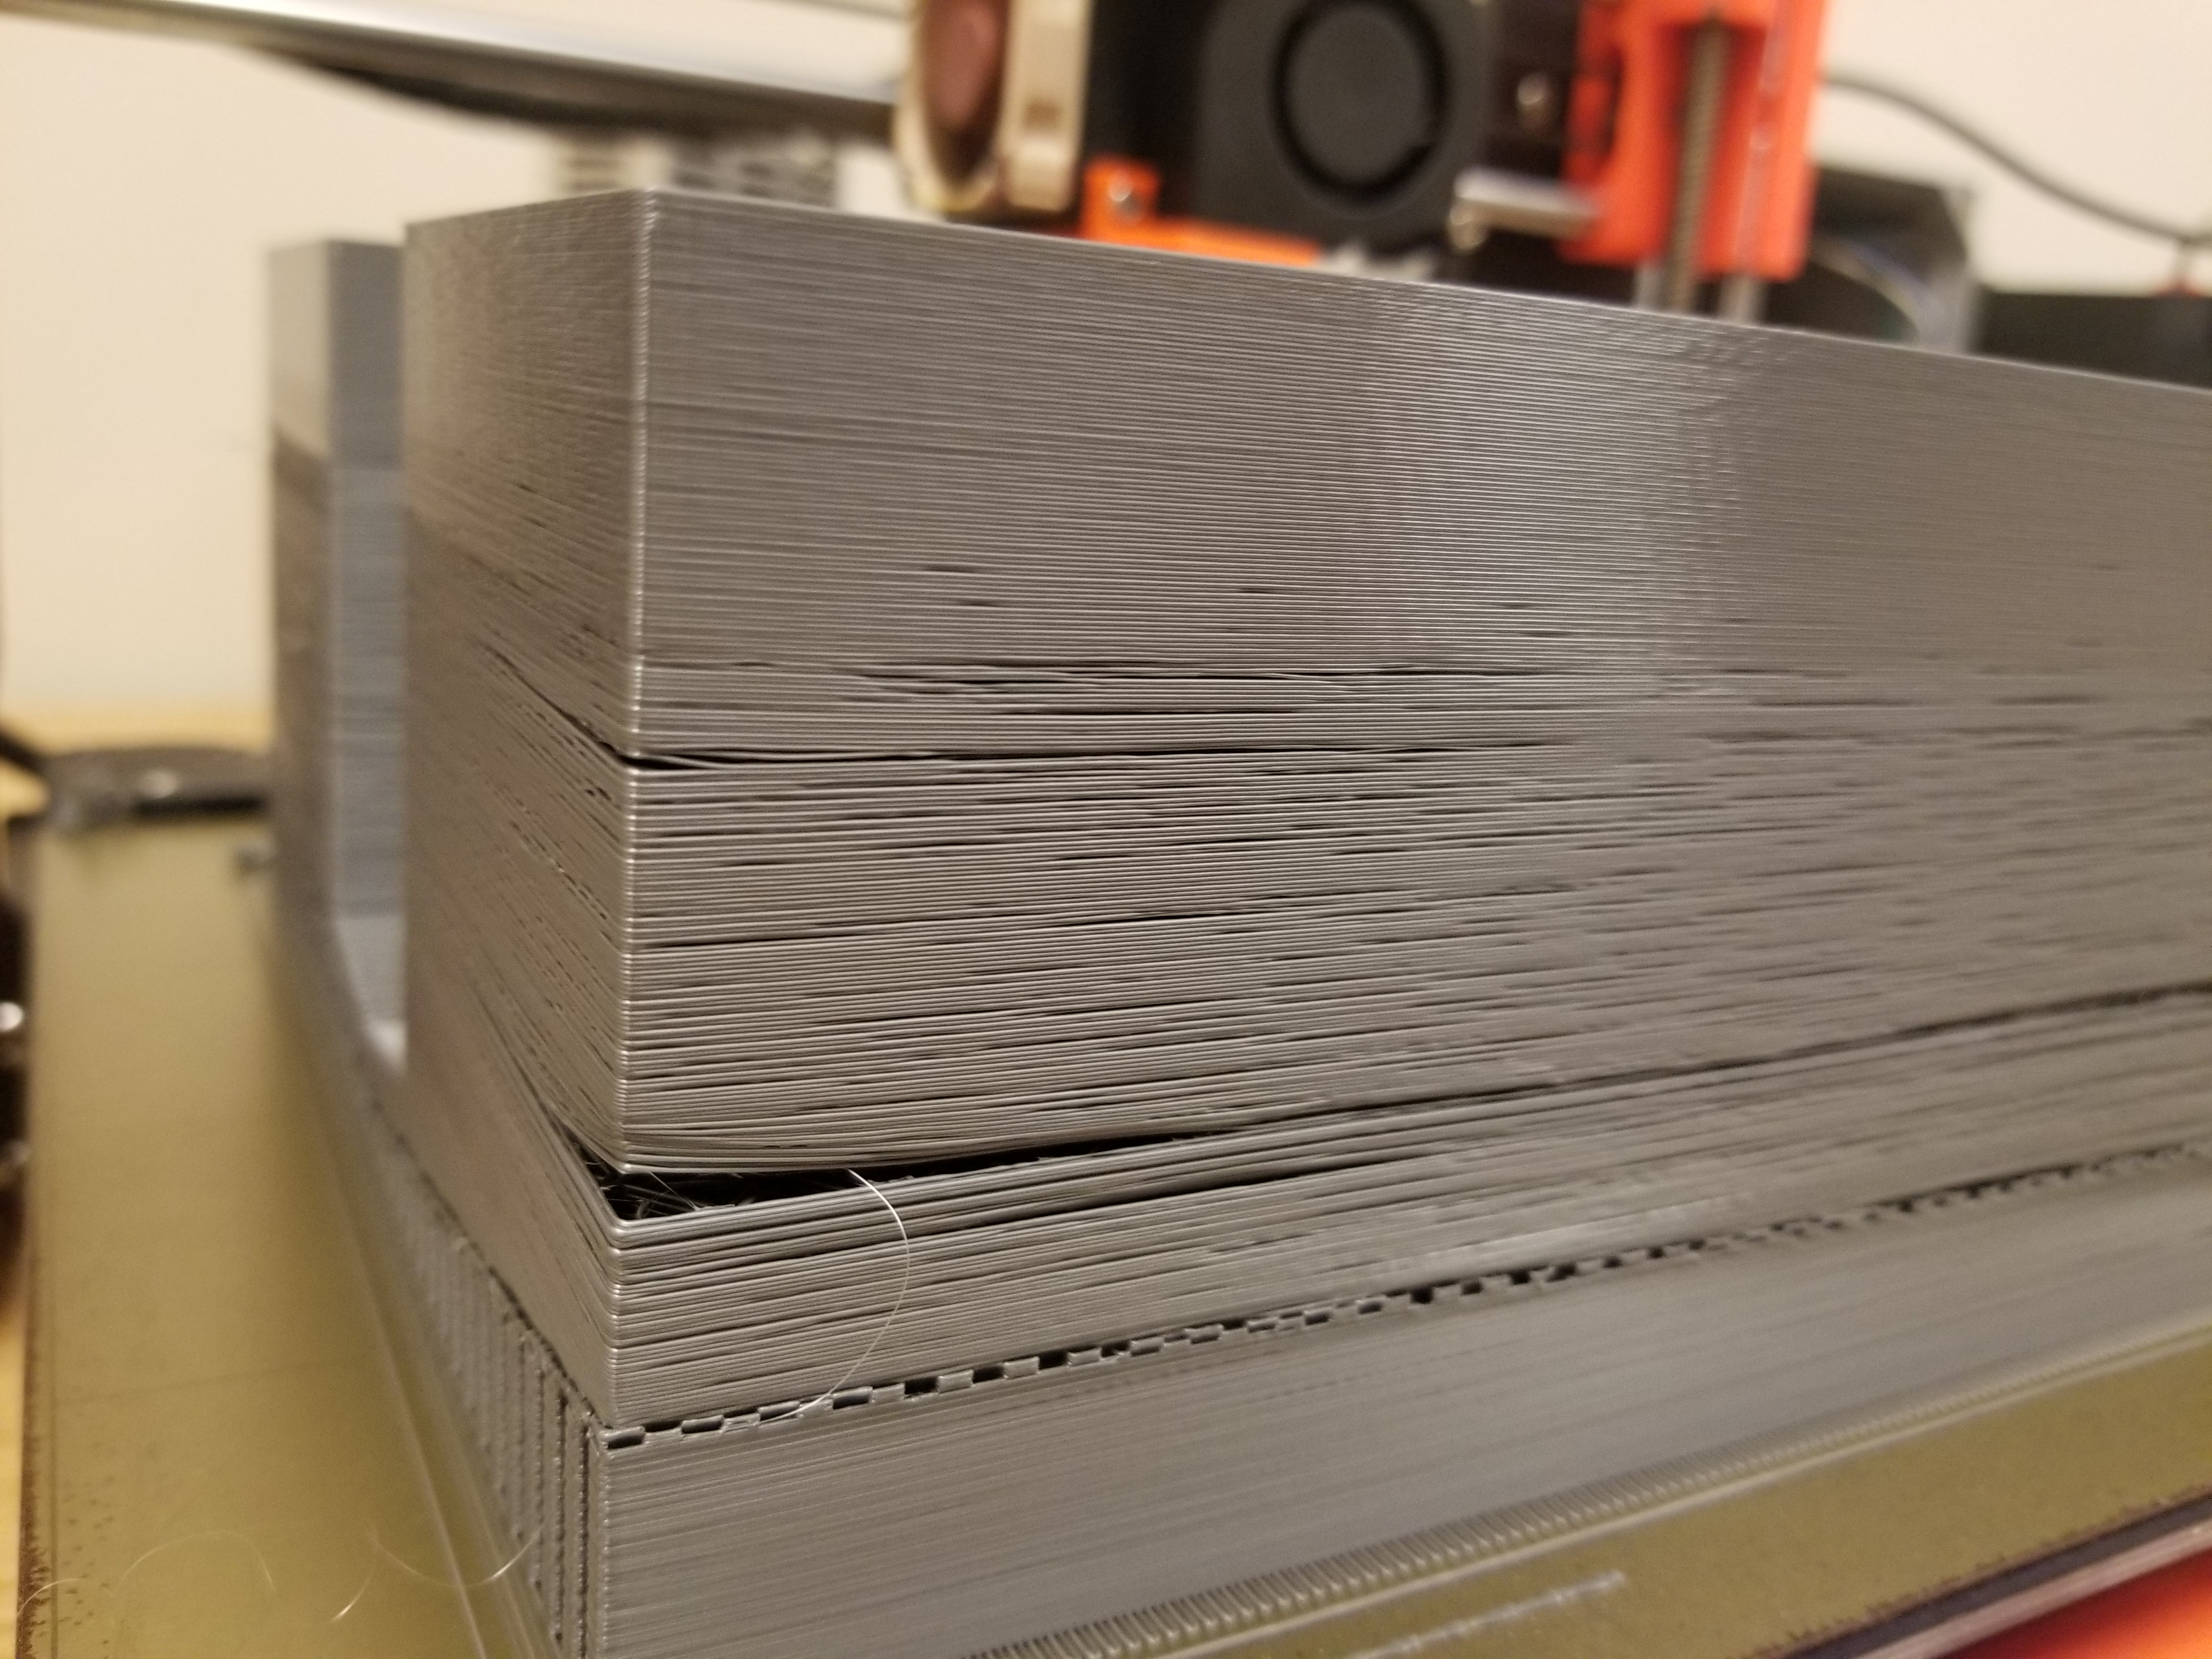
\includegraphics[width=\textwidth]{24382-129778-20190220-061954.jpg}
        \caption{Layers split issue\cite{onlineOpenSource2}}
        \label{fig:image2}
    \end{subfigure}
    \hfill

    \caption{Two types of 3D printing issues}
    \label{fig:test}
\end{figure}

\newpage

\section{Data Processing}
\subsection{Dataset Structure}
The dataset includes images of the defect and corresponding labels. The directory structure is organized into training and validation sets.
\\
Directory tree:
{\dirtree{%
.1 data/.
.2 images/.
.3 train/.
.4 ....
.3 val/.
.4 ....
.2 labels/.
.3 train/.
.4 ....
.3 val/.
.4 ....
}}


\subsection{Labeling Importance}
Labels are crucial for training the YOLO algorithm. They provide information on object location and class within the images. 
\subsection{Labeling Process}
We use {\textbf {MakeSense}}{ \scriptsize \cite{labelingTool3}}, a free online tool, for labeling images. Labels are exported in YOLO format.

\begin{figure}[h]
    \centering
    \begin{subfigure}[b]{0.45\textwidth}
        \centering
        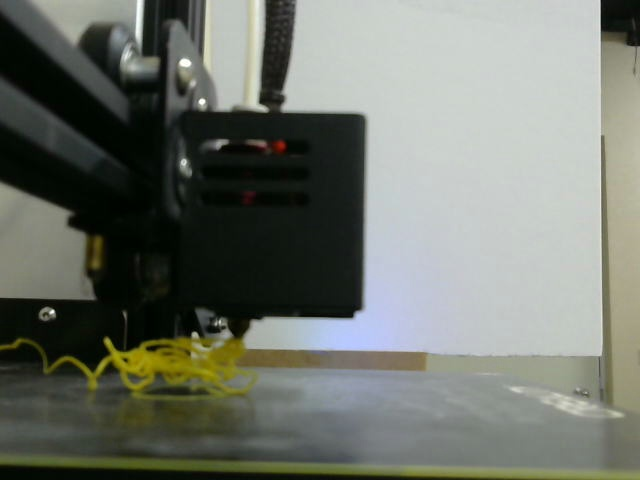
\includegraphics[width=\textwidth]{no_support_62.jpg}
        \caption{no\_support\_62.jpeg \cite{onlineOpenSource2}}
        \label{fig:image1}
    \end{subfigure}
    \begin{subfigure}[b]{0.45\textwidth}
        \centering
        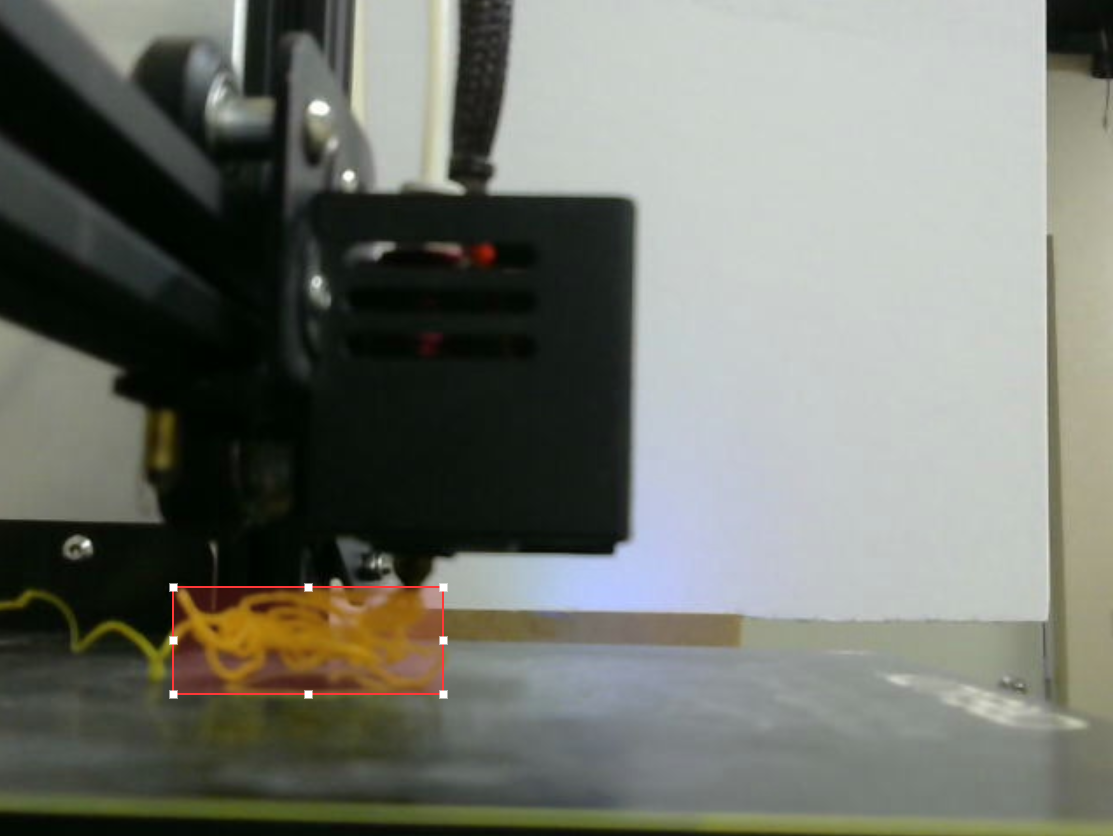
\includegraphics[width=\textwidth]{LabelByMakeSens.png}
        \caption{no\_support\_62.jpeg (labeled)\cite{onlineOpenSource2}}
        \label{fig:image2}
    \end{subfigure}
    \hfill
    \caption{Comparison of image without and with label}
    \label{fig:test}
\end{figure}

\newpage

\section{Conclusion}
This simplified process ensures the preparation of a relevant dataset, enabling the YOLO algorithm to effectively detect the "spaghetti" defect in 3D printing.his simplified process ensures the preparation of a relevant dataset, enabling the YOLO
algorithm to effectively detect the ”spaghetti” defect in 3D printi


\begin{thebibliography}{9}

    \bibitem{onlineOpenSource1}
        Dataset: \href{https://www.kaggle.com/datasets/justin900429/3d-printer-defected-dataset}{3D-Printer Defected Dataset}: \\
        {\footnotesize \url{https://www.kaggle.com/datasets/justin900429/3d-printer-defected-dataset}}
    \bibitem{onlineOpenSource2}
        Dataset: \href{https://www.kaggle.com/datasets/mikulhe/3d-printing-errors}{3D printing errors}: \\
        {\footnotesize \url{https://www.kaggle.com/datasets/mikulhe/3d-printing-errors}}
    \bibitem{labelingTool3}
        MakeSense: \href{https://www.makesense.ai/}{MakeSense}: \\
        {\footnotesize \url{https://www.makesense.ai/}}

    \end{thebibliography}

\end{document}
